%%% start preambling . . .  %%%
\documentclass{article}

% required 
\usepackage{Sweave}
\usepackage{graphicx}


% https://tex.stackexchange.com/questions/60209/how-to-add-an-extra-level-of-sections-with-headings-below-subsubsection
\usepackage{titlesec}
\setcounter{secnumdepth}{4}

\titleformat{\paragraph}
{\normalfont\normalsize\bfseries}{\theparagraph}{1em}{}
\titlespacing*{\paragraph}
{0pt}{3.25ex plus 1ex minus .2ex}{1.5ex plus .2ex}



% recommended! Uncomment the below line and change the path for your computer!
 
%put your figures in one place! Also, note that here 'figures' is the folder and 'demoFig' is what each 
% figure produced will be titled plus its number or label (e.g., demoFig-nqpbetter.pdf')

% make your captioning look better
\usepackage[small]{caption}
\setlength{\captionmargin}{30pt}
\setlength{\abovecaptionskip}{0pt}
\setlength{\belowcaptionskip}{10pt}

% optional: muck with spacing
\topmargin -1.5cm        
\oddsidemargin 0.5cm   
\evensidemargin 0.5cm  % same as oddsidemargin but for left-hand pages
\textwidth 15.59cm
\textheight 21.94cm 
% \renewcommand{\baselinestretch}{1.5} % 1.5 lines between lines
\parindent 0pt		  % sets leading space for paragraphs
% optional: cute, fancy headers
\usepackage{fancyhdr}
\pagestyle{fancy}
\fancyhead[LO]{November 2022}
\fancyhead[RO]{Manuscript}
% more optionals! %
\usepackage[hyphens]{url} % this wraps my URL versus letting it spill across the page, a bad habit LaTeX has

%%% end preambling. %%%

\begin{document}
\Sconcordance{concordance:supplement.tex:supplement.Rnw:%
1 65 1}
 % For RStudio hiccups
\title{{\huge Changes and trends in budburst and leaf flush across Europe and North America} \\A meta-analysis of local adaptation in spring phenology studies}
\author{Ziyun Zeng \& E. M. Wolkovich}
\date{November 2022}
\maketitle 


\newpage

\section*{Abstract}
\section{Introduction}

\begin{itemize}
\item Define spring event, fall event
\item Background
\item Research question (links to results)
\end{itemize}

\section{Methods}
\begin{itemize}
\item Literature search
\item Provenance location and spring/fall DOY data gathering using ImageJ
% note that we primarily focused on papers with spring data
  \begin{itemize}
\item Read SB 2015 and A 2013, took paper with spring doy and provenance coordinates from them
\item Searched online for more papers (explain criteria here)
\item Out of 59 papers related to common garden/spring phenology that I read, only 22 can supply data that we need; Out of the 22, 4 studies have provenance and gardens on different continents, which were subsequently archived (can document in supplements)).
\end{itemize}
\item Present how many gardens, species, provenance we have using a table, which also documents the type of spring event they looked at, year, etc. 
\item Insert mapped locations of studies
\item Climate data gathering
  \begin{itemize}
  \item Simple climate matrix (MAT \& MSP/MAP) gathering
  \begin{itemize}
  \item ClimateNA by Dr. Tongli Wang
  \item Climate Information Tool by FAO
  \end{itemize}
  \item Daily climate data gathering: Gridded daily climate data downloaded for all provenances and gardens: We hope that coarse metrics such as latitude and MAT ultimately represent how similar the climates are between the provenances and gardens in times that matter for the events. If climates are very similar, then we would expect similar timings [add more here].
To this end, we estimated climate overlap in relevant months: For spring events, we considered overlap across March to May.
  \begin{itemize}
  \item North American daily climate data from Daymet R package
  \item Europe daily climate data (gridded: NetCDF-4) retrieved from E-OBS 
  \end{itemize}
  \end{itemize}
  \item Estimate climate overlap using daily climate data using Overlap R package
  \item Calculated GDDs, spherical distances
  \item Corrected for DOY (taking the difference), will put results in supplement
  \item Mixed effects modelling: We used hierarchical Bayesian models where we partially pooled by species. We estimated effects of continent and species type (angiosperm VS gymnosperm) from posterior estimates, in relation to single predictors (including provenance latitude, MAT) and two predictors (climate overlap percentage and standard deviation).
\end{itemize}

\section{Results}
%AZZNov04: all subsection titles are placeholders

\subsection{Provenance latitude and MAT do not affect spring event timing}

Overall, our models show that spring events are not related to provenance latitude or mean annual temperature in North America, and only weakly related in Europe (Figure \#). 
\\
\verb@Alina Says: Need to elaborate here. Note that all figures are subject to update for better resolution. I might add climate overlap plots here too.@

\begin{figure}[!h] 
    \centering
 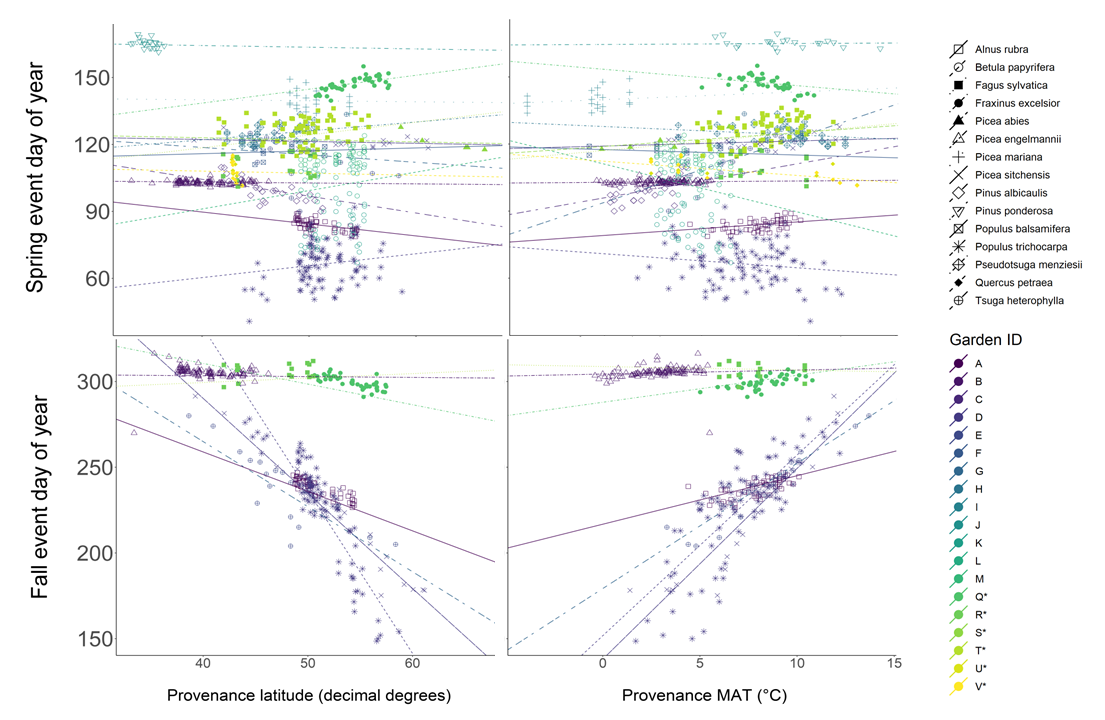
\includegraphics[width=\textwidth]{..//..//localadaptclim/Docs/figure_ms/springfall_latmat.png}
    \caption{Spring event Day of Year (DOY) in relation to provenance latitude and MAT, coded by symbol for species and color for garden with linear fits from hierarchical Bayesian models. Spring events shown on top and fall event at the bottom.}
    \label{figure:springfall_latmat}
\end{figure}


\newpage

\subsubsection {Similar results across provenance latitude, latitude difference, and distance}
\verb@Alina says: need to find a name for each metric and stick to it.@
Along with (a) provenance latitude, we also looked at how spring event timing is related to (b) the absolute difference between provenance latitude and garden latitude , as well as (c) the spherical distance between the garden and each provenance. All three metrics depict little to no relationship between spring event timing and the geographical location of the provenance \verb@(Supplement Figure #)@.
% can show that figure in supplement

\subsubsection {Climate overlap does not predict event dates much better than provenance latitude or MAT}

While comparing how similarity in climate relates to event dates, we observed very weak effects of climate overlap on spring events, nearly identical across angiosperms and gymnosperms. Fall events diverge as climate overlap declines for both angiosperms and gymnosperms, but slightly more strongly for gymnosperms.
% add figure here

\subsubsection {Strong relationship between provenance latitude, MAT, and GDDs}

I am unsure about how to commment on what we are seeing in this plot. There is a strong relationship between GDDs of each event day recorded and the latitude and MAT, but isn't that self-apparent? also I don't know how to link (Fig. \#) in text with the corresponding figure being displayed. 

% all figures will be updated (color, font size, resolution)
\begin{figure}[!h] 
    \centering
 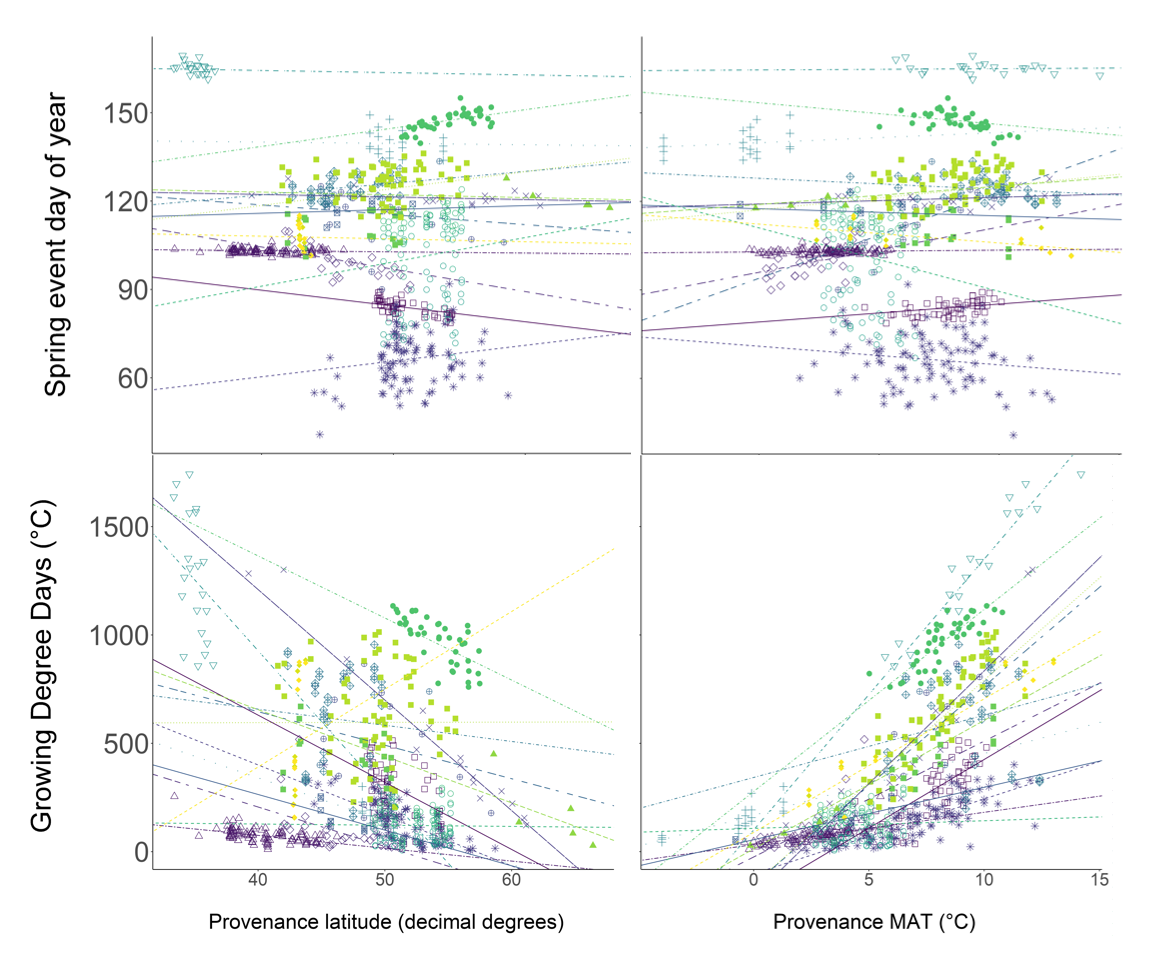
\includegraphics[width=\textwidth]{..//..//localadaptclim/Docs/figure_ms/gdd_ms.png}
    \caption{Growing Degree Days (GDD)on each day of spring event in relation to provenance latitude and MAT, coded by symbol for species and color for garden with linear fits from hierarchical Bayesian models.}
    \label{figure:gdd}
\end{figure}


\newpage


\subsection{Stronger clines in fall events observed in North America than Europe}

% old graphs can be found in C:\Users\alina\Documents\git\localadaptclim\Output\plotMay15_two predictors_experiment
% refer to analyses\script_model_continent_spp_type_effect
% https://github.com/lizzieinvancouver/localadaptclim/issues/16

% need to replot ofc


%  extract the mean estimate of the slope and report that instead of ~4 or such
% hmmm i forgot the code :)))

We find that fall events (budset, leaf senescence, leaf abcission) advance strongly with provenance latitude and mean annual temperature, meaning fall events are earlier where provenance mean annual temperature is lower (higher, more northern latitudes). This relationship, however, is observed mostly in North America where fall events advance 4.2 days per degree we move north, or 6.4 days when the MAT decreases by one $^{\circ}$C. In Europe, such relationship is weak: advance 0.5 days per degree we move north, or 0.6 days when the MAT decreases by one $^{\circ}$C.
% add figure here

\subsection{Effects of MAT on spring events diverge across angiosperms and gymnosperms}

Effects of provenance latitude on both spring and fall events are similar across angiosperms and gymnosperms. However, effects of MAT on spring events weakly diverge: spring events get earlier as MAT increases in angiosperms and delay as MAT increases in gymnosperms, except for \emph{Pseudotsuga menziesii}. Fall events delay in warmer locations for both species types, but slightly more so for gymnosperms (3.7 days VS. 6.2 days).


\section{Discussion}




The weak relationship between spring event dates and provenance latitude and MAT that we find in European studies might be explained by the higher extent of climate overlap in those studies. The more similar the climate is between provenances and gardens, the less difference between spring event dates.
\\

The inconsistent and weak clines in spring events that we found suggest high plasticity in spring phenology across continents and species. Fall events, on the other hand, exhibit stronger clines which suggest more local adaptation, especially in North America. Overall, our results predict that warming springs will continue to be tracked more closely phenologically by trees than warming fall temperatures.
\\

In contrast to spring events, we found strong latitudinal clines in fall events across both continents, with local adaptation appearing much stronger in North America than in Europe. Our results show that spring events are highly plastic, and thus may shift with warming, but data on more species and greater information on important factors, such as their geographic location in relation to their origins and elevation, are needed for forecasting. 



\bibliography{..//..//refs/ranges}
\section{Figures}



\end{document}



% formatting code resources
% https://github.com/lizzieinvancouver/ospree/blob/master/docs/ranges/ranges_outline.tex
% https://github.com/lizzieinvancouver/ospree/blob/master/docs/traits/Traitors_Manuscript_supp.Rnw

